\chapter{Introduzione}%
\label{cha:Introduzione}
In questo capitolo vengono introdotti i concetti base dei problemi di
ottimizzazione, i problemi di programmazione lineare (LP), i problemi
di programmazione lineare intera mista (MIP) e i rispettivi algoritmi
risolutivi.

\section{Definire un problema di ottimizzazione}
\label{sec:Introduzione}
Un problema di ottimizzazione $P$ viene definito come segue:
\begin{equation}
    P:
    \begin{cases}
        \min (\textit{or} \max)f(x)\\
        S\\
        x \in D
    \end{cases}
\end{equation}
dove $x$ è una tupla $(x_1, \ldots, x_n)$, $D$ è un prodotto cartesiano 
$D_1 \times \ldots \times D_n$ tale per cui $x_j \in D_j\,\forall j = 1,\ldots,n$,
$f(x)$ è una funzione a valori reali in $x$ ed infine $S$ è un insieme finito 
di vincoli.

Un vincolo $c \in S$ può essere una disuguaglianza o un'uguaglianza ed è
associato ad un sottoinsieme di variabili $x_c$.
Si parla di vincolo soddisfatto quando il suo valore è vero, in caso contrario
si parla di vincolo violato.

Ogni $x\in D$ viene chiamata \textit{soluzione} di $P$; se $x$ soddisfa i tutti i 
vincoli del problema allora la soluzione viene detta \textit{ammissibile}. 
L'insieme delle soluzioni ammissibili di un problema di ottimizzazione 
$P$ si indica con $F(P)$.

Un problema di ottimizzazione viene detto \textit{impossibile} (\textit{infeasible})
se $F(P) = \varnothing$; \textit{illimitato} (\textit{unbounded})
se $f(x)$ non presenta un limite inferiore per una qualsiasi $x \in F(P)$.
Infine si dice che un problema \textit{ammette ottimo finito} se esiste almeno
una \textit{soluzione ottima} $x^*\in F(P)$.
Una soluzione $x^*\in F(P)$ è ottima se
\begin{equation}
    f(x^*) \leq f(x) \quad \forall x \in F(P).
\end{equation}

Risolvere un problema di ottimizzazione significa trovare una \emph{soluzione
ottima}, dimostrare che sia tale oppure dimostrare che il problema è impossibile
o illimitato.

\section{Concetti generali dell'ottimizzazione}%
\label{sec:Concetti generali dell'ottimizzazione}
Introduciamo i concetti sui quali si basano gli algoritmi risolutivi.

\subsection{Ricerca}%
\label{sub:Ricerca (search)}
Effettuare una ricerca consiste nel risolvere una sequenza 
di restrizioni $P_1, \ldots, P_m$ di un problema $P$. 
Una restrizione $P_k$ è un problema di ottimizzazione ottenuto da $P$ aggiungendo
dei vincoli.
Si osserva che:
\begin{enumerate}
    \item se $F(P_k)$ è illimitato allora lo è anche $F(P)$;
    \item se $F(P_k) = \varnothing$, ovvero se $P_k$ è impossibile,
        allora non si può dire nulla di $F(P)$;
    \item se $F(P_k)$ presenta una soluzione ottima allora abbiamo trovato
        il limite superiore della soluzione ottima di $P$.
\end{enumerate}
Notiamo come, nell'ultimo caso, abbiamo ricavato un'informazione sulla soluzione
ottima di $P$ risolvendo una sua restrizione.

%\begin{figure}[ht!]
%\begin{center}
%    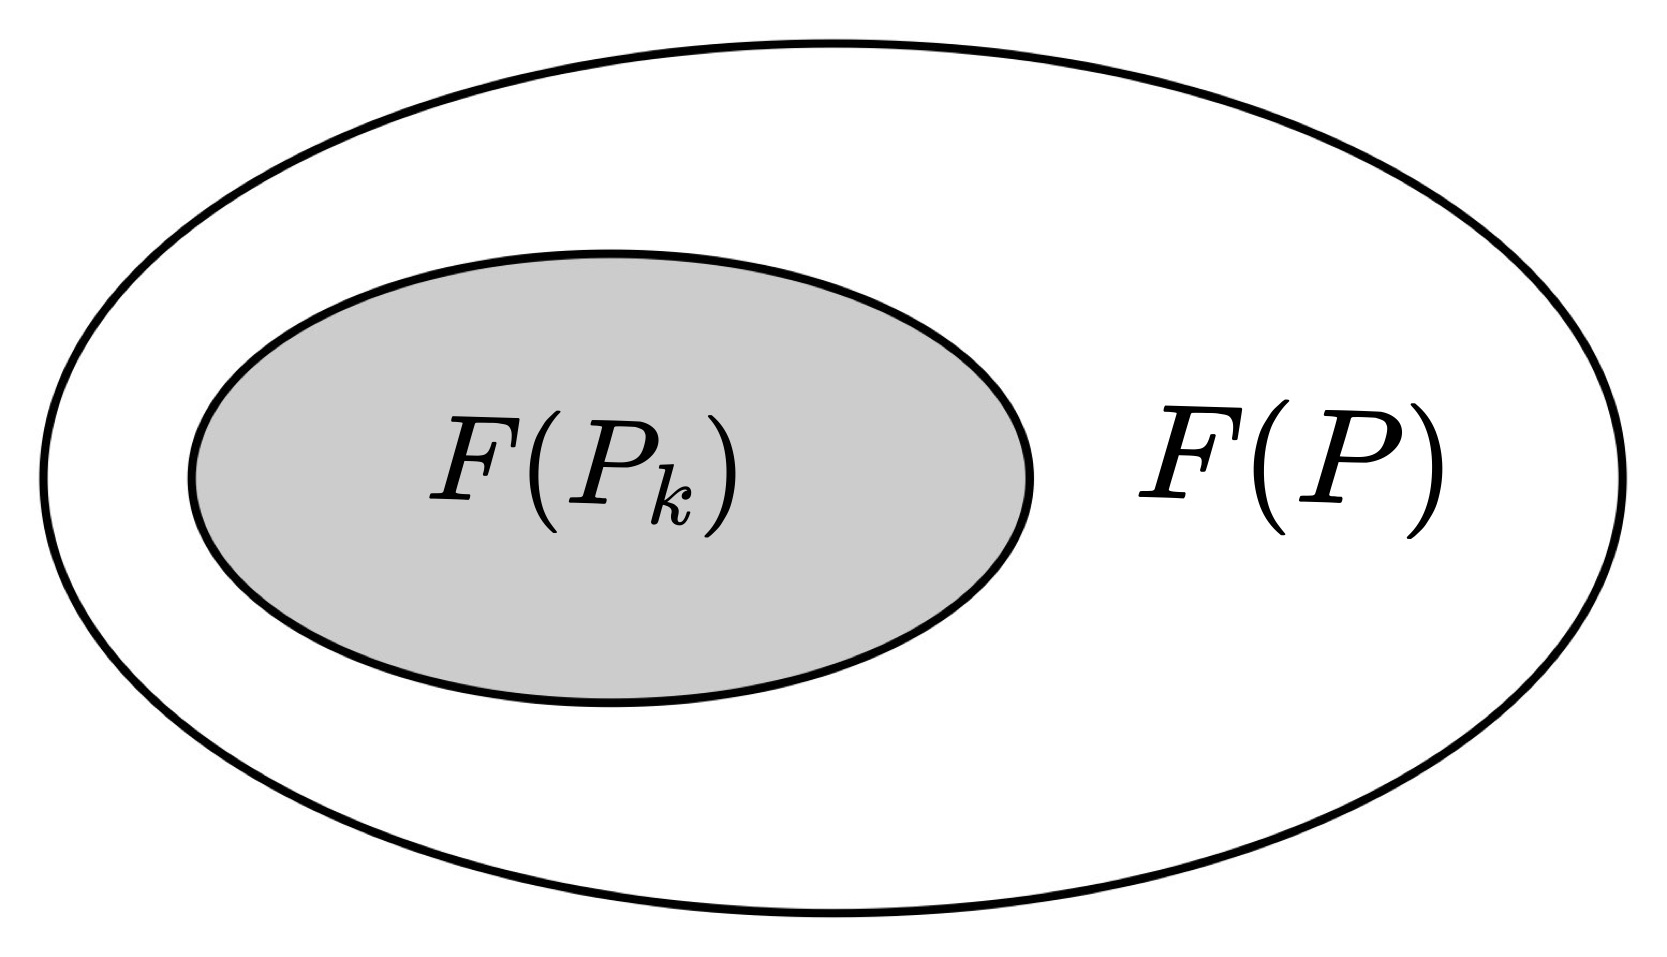
\includegraphics[scale=0.06]{img/restrizione}
%    \caption{L'insieme delle soluzioni ammissibili di $P_k$ è un
%    sottoinsieme dell'insieme delle soluzioni ammissibili di $P$.}
%\end{center}
%\end{figure}

\noindent
Una ricerca viene detta \textit{esaustiva} quando l'insieme delle restrizioni
$P_k$ ricopre l'intero spazio delle soluzioni ammissibili di $P$, ovvero 
$\bigcup_i F(P_i) = F(P)$.
L'esempio più semplice di algoritmo di ricerca esaustivo è il \textit{generate
and test}.
L'algoritmo ricava tutte le soluzioni $x \in D$, verifica quali di queste
soddisfa i vincoli del problema ed infine sceglie la migliore.
In questo caso le restrizioni di $P$ si ottengono fissando
$x$ ad un certo valore appartenente al dominio $D$.
Per come lo abbiamo descritto, l'algoritmo è esponenziale.
Tuttavia può risultare efficace se utilizzato in casi specifici,
per esempio quando le possibili soluzioni del problema non sono 
in numero elevato e sono computazionalmente poco costose.

Un algoritmo di ricerca esaustiva più avanzato è la \textit{ricerca ad albero}.
L'algoritmo divide ricorsivamente lo spazio di ricerca di $P$ fino ad ottenere
delle restrizioni (corrispondenti alle foglie dell'albero) sufficientemente
facili da risolvere.
Il caso peggiore ha prestazioni esponenziali e si verifica quando tutte le 
foglie corrispondono a restrizioni di $P$ in cui $x$ è fissato ad un valore 
appartenente al dominio $D$, in altre parole l'algoritmo diventa identico
al generate and test.
L'algoritmo per la risoluzione di problemi di programmazione lineare intera 
che introdurremo successivamente, si basa sulla ricerca ad albero.

L'ultima tipologia di ricerca che introduciamo è quella \emph{euristica}.
La ricerca euristica permette di ottenere una soluzione del problema $P$
più velocemente rispetto ad una ricerca esaustiva.
Il vantaggio di questo approccio è proprio la velocità mentre lo svantaggio
principale è che in generale gli algoritmi euristici non sono ottimi, ovvero
non trovano una soluzione ottima ma ne trovano una ammissibile.
L'ACS si basa sulla ricerca euristica.

\subsection{Rilassamento}%
\label{sub:Rilassamento}
Un rilassamento di un problema di ottimizzazione $P$ è un altro problema 
di ottimizzazione $R$ ottenuto da $P$ eliminando alcuni vincoli e sostituendo 
la funzione obiettivo $f(x)$ con una sua approssimazione inferiore $g(x)$.
In altre parole: $R$ è un rilassamento di $P$ se $F(P) \subseteq F(R)$ e se
$g(x) \leq f(x) \quad \forall x \in F(P)$.
Valgono le seguenti proprietà:
\begin{itemize}
    \item se $F(R) = \varnothing$ allora  $F(P) = \varnothing$;
    \item se $x^*$ è una soluzione ottima di $R$, allora $g(x^*)$ è un limite
        inferiore valido per il valore ottimo di $P$.
    \item se $x^*$ è una soluzione ottima di $R$, $x^* \in F(P)$ e $g(x^*) = f(x^*)$,
        allora $x^*$ è ottima anche per $P$.
\end{itemize}

%\begin{figure}[ht!]
%\begin{center}
%    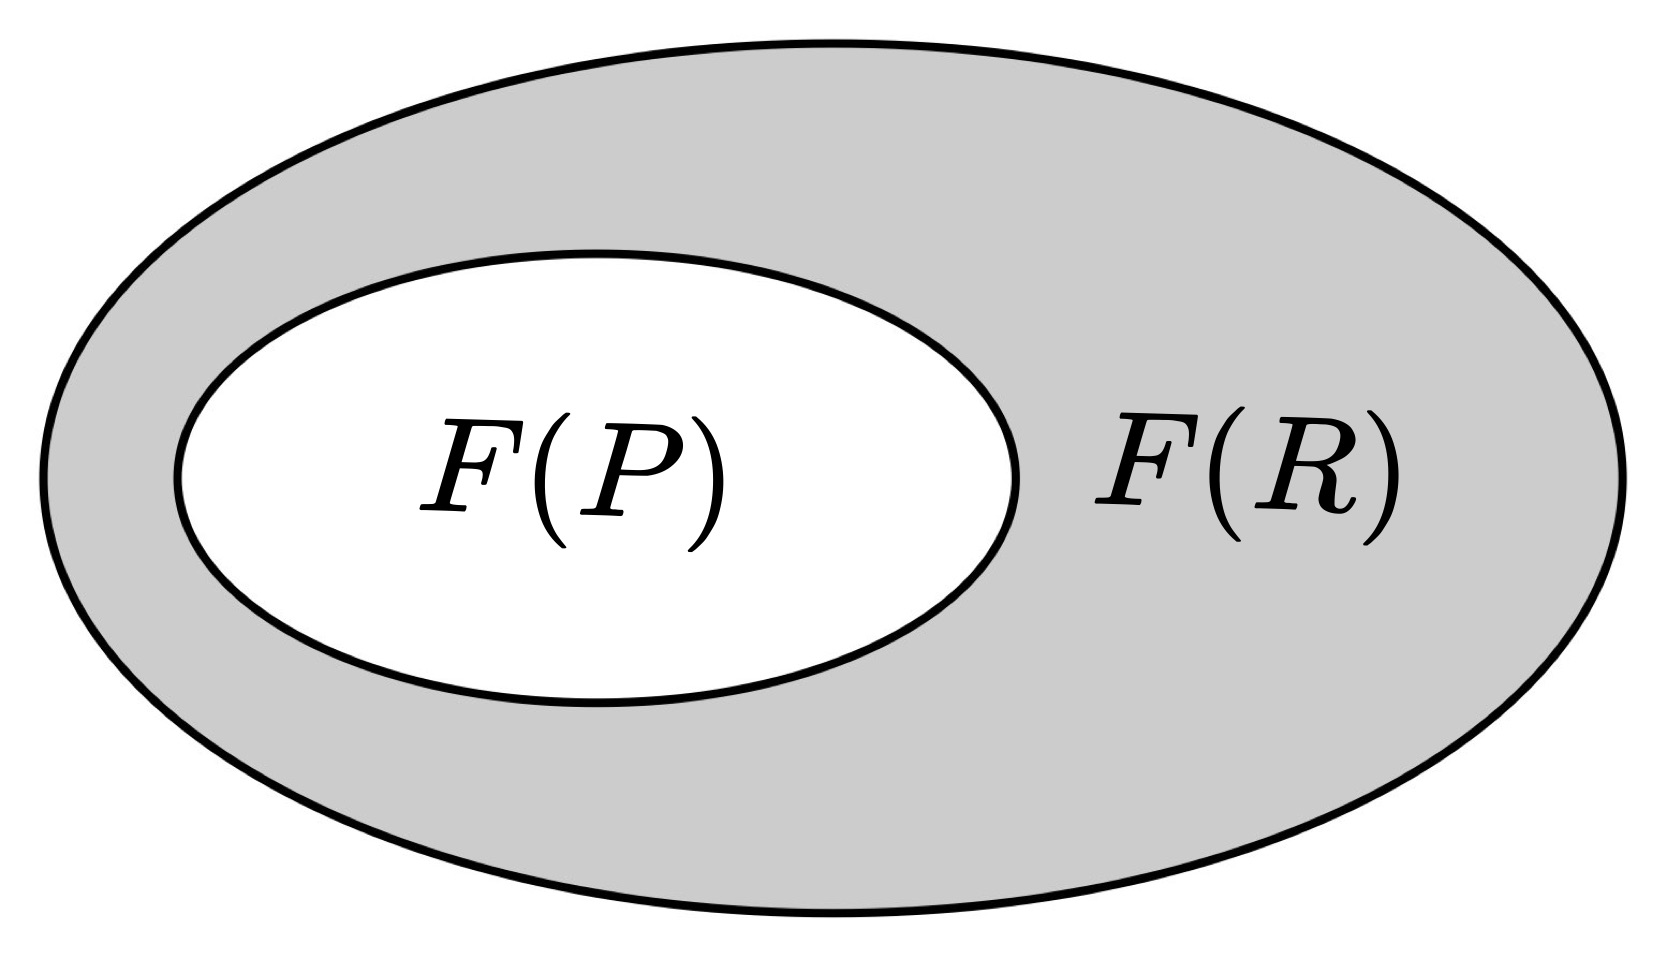
\includegraphics[scale=0.06]{img/relax}
%    \caption{L'insieme delle soluzioni ammissibili di $P$ è un sottoinsieme
%    dell'insieme delle soluzioni ammissibili di $R$.}
%\end{center}
%\end{figure}

\section{Programmazione lineare}%
\label{sec:Programmazione lineare}
Un generico problema di programmazione lineare è definito come segue:
\begin{equation} \label{eq:lpDef}
    P:
    \begin{cases}
        \min\,c^tx\\
        a_ix \sim b_i & i=1,\ldots,m\\
        l_j \leq x_j \leq u_j & j = 1, \ldots, n
    \end{cases}
\end{equation}
dove $\sim \in \{\leq, \geq, =\}$, $l_j \in \R \cup \{-\infty\}$ e $u_j \in \R \cup 
\{+\infty\}$ e dove $c^tx$ è funzione lineare.
Le disuguaglianze strette non sono permesse, ciò è dovuto al fatto che 
gli algoritmi che risolvono questa tipologia di problemi richiedono che le 
soluzioni ammissibili appartengano ad un insieme chiuso.
Più avanti vedremo il perché di questa scelta.

Dato un problema di programmazione lineare, esiste un algoritmo che, al caso peggiore,
riesce a risolverlo con complessità polinomiale nella taglia del problema.
La taglia di un problema è definita dal numero delle variabili e di vincoli.

In generale la programmazione lineare è poco applicabile in quanto la maggior
parte dei problemi reali non rientra a far parte di questa categoria.
Sebbene non venga spesso applicata direttamente, risulta essere uno strumento
di fondamentale importanza che viene utilizzato da algoritmi che risolvono
problemi più complessi.

% TODO: Algoritmo del Simplesso.

\section{Programmazione lineare intera}%
\label{sec:MIP intro}
Un problema di programmazione lineare intera (MIP, \emph{Mixed Integer linear 
Programming}) è definito come segue:
\begin{equation}
    P:
    \begin{cases}
        \text{min}\,cx\\
        a_ix \sim b_i & i=1,\ldots,m\\
        l_j \leq x_j \leq u_j & j = 1, \ldots, n = N\\
        x_j \in \Z & \forall j \in J\subseteq N = \{1,\ldots, n\}
    \end{cases}
\end{equation}
dove $\sim \in \{\leq, \geq, =\}$.
Troviamo gli stessi vincoli che si trovano in \ref{eq:lpDef},
in aggiunta è presente il vincolo che alcune delle variabili devono assumere
valori interi.

Si riescono a modellare molti più problemi con la programmazione lineare
intera rispetto alla programmazione lineare.

\subsection{Algoritmo Branch and Bound}%
\label{sub:Algoritmo Branch And Bound}
Il branch-and-bound (B\&B) è un algoritmo che si basa sul paradigma 
divide-and-conquer, viene utilizzato per risolvere problemi di ottimizzazione 
generica tra cui i problemi di programmazione lineare intera.
Il B\&B implementa una ricerca ad albero che permette di 
ricavare una soluzione ottima del problema considerato.

L'algoritmo inizia dal nodo radice il quale rappresenta il problema MIP $P$
che vogliamo risolvere.
\begin{enumerate}
    \item Si considera il rilassamento $R$ di $P$ ottenuto rimuovendo 
        il vincolo di interezza sulle variabili. $R$ è un problema di programmazione 
        lineare ed è quindi più semplice da risolvere.
        Si possono presentare tre casi:
        \begin{enumerate}
            \item Se $F(R) = \varnothing$ allora $F(P) = \varnothing$ quindi
                l'algoritmo termina.
            \item Se esiste una soluzione ottima $x^*\in F(R)$ tale per cui $x^* \in F(P)$,
                allora $x^*$ è ottima per $P$ e l'algoritmo termina.
            \item Se invece $x^* \notin F(P)$ significa che 
                la soluzione trovata non rispetta almeno un vincolo di interezza,
                allora abbiamo trovato un \emph{limite inferiore} sull'ottimo di $P$.
        \end{enumerate}
        Se ci ritroviamo nel caso $(c)$ allora l'algoritmo prosegue.

    \item Si effettua \emph{branching} sul nodo radice.
        L'operazione di branching applicata ad un nodo permette di individuare
        i suoi nodi figli: questi sono sottoproblemi che vengono
        ottenuti mediante restrizioni del problema genitore.
        Almeno una delle variabili della soluzione $x^*$ non rispetta il vincolo
        di interezza, ovvero
        $ \exists\,j \in J \,:\, x^*_j \notin \Z$.
        Di conseguenza due nodi figli possono essere creati imponendo a ciascuno
        uno dei seguenti due vincoli aggiuntivi:
        \begin{equation}
            x_j \leq \lfloor x^*_j \rfloor,\quad x_j \geq \lceil x^*_j \rceil.
        \end{equation}
        I nodi vengono aggiunti alla coda $Q$ dei sottoproblemi da risolvere.
        La Figura~\ref{fig:branching} mostra il risultato di un'operazione di
        branching dal punto di vista della regione ammissibile del problema $P$.

        \begin{figure}[ht!]
            \begin{center}
                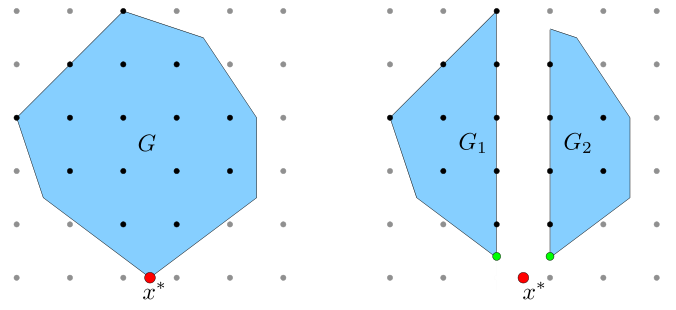
\includegraphics[scale=0.4]{./img/branching.png}
            \end{center}
            \caption{Operazione di branching dal punto di vista della
            regione ammissibile.}
            \label{fig:branching}
        \end{figure}

    \item Si procede considerando un sottoproblema $P_i \in Q$ e si risolve
        un suo rilassamento $R_i$.
        Possono verificarsi quattro casi:
        \begin{enumerate}
            \item Se $F(R_i) = \varnothing$ allora il nodo può essere scartato
                (\emph{prouning by infeasibility}).
            \item Se esiste una soluzione ottima $\overline{x}\in F(R_i)$
                tale che $\overline{x} \in F(P_i)$ allora abbiamo trovato un limite
                superiore $\overline{z} = c \overline{x}$ valido per la 
                soluzione ottima di $P$. $\overline{z}$ viene chiamato
                \emph{incumbent}: si tratta della migliore soluzione attuale di
                $P$.
            \item Se $\overline{x} \notin F(P_i)$, si confronta l'incumbent
                con la soluzione trovata: se $c \overline{x} \geq \overline{z}$
                allora il nodo può essere scartato (\emph{prouning by optimality})
                in quanto $c \overline{x}$ è il limite inferiore sull'ottimo
                di $P_i$, pertanto non può portare ad una soluzione migliore
                dell'attuale incumbent.
            \item Altrimenti ($c \overline{x} < \overline{z}$)
                è necessario fare branching sul nodo ed aggiungere i suoi
                figli a $Q$.
        \end{enumerate}

    \item Il più piccolo valore tornato dai rilassamenti dei nodi aperti è un
        limite inferiore valido per la soluzione ottima di $P$.
        Sfruttando questa proprietà viene aggiornato il valore del limite
        inferiore trovato nel primo punto.

    \item L'algoritmo procede finché la coda dei sottoproblemi $Q$ si svuota.
        In questa situazione il valore dell'incumbent coincide con quello
        del limite inferiore e pertanto $\overline{z}$ corrisponde alla
        soluzione ottima di $P$ trovata dall'algoritmo.
\end{enumerate}

% TODO: Metto la figura dell'andamento dell'upper e lower bound?
\begin{figure}[ht!]
\begin{center}
    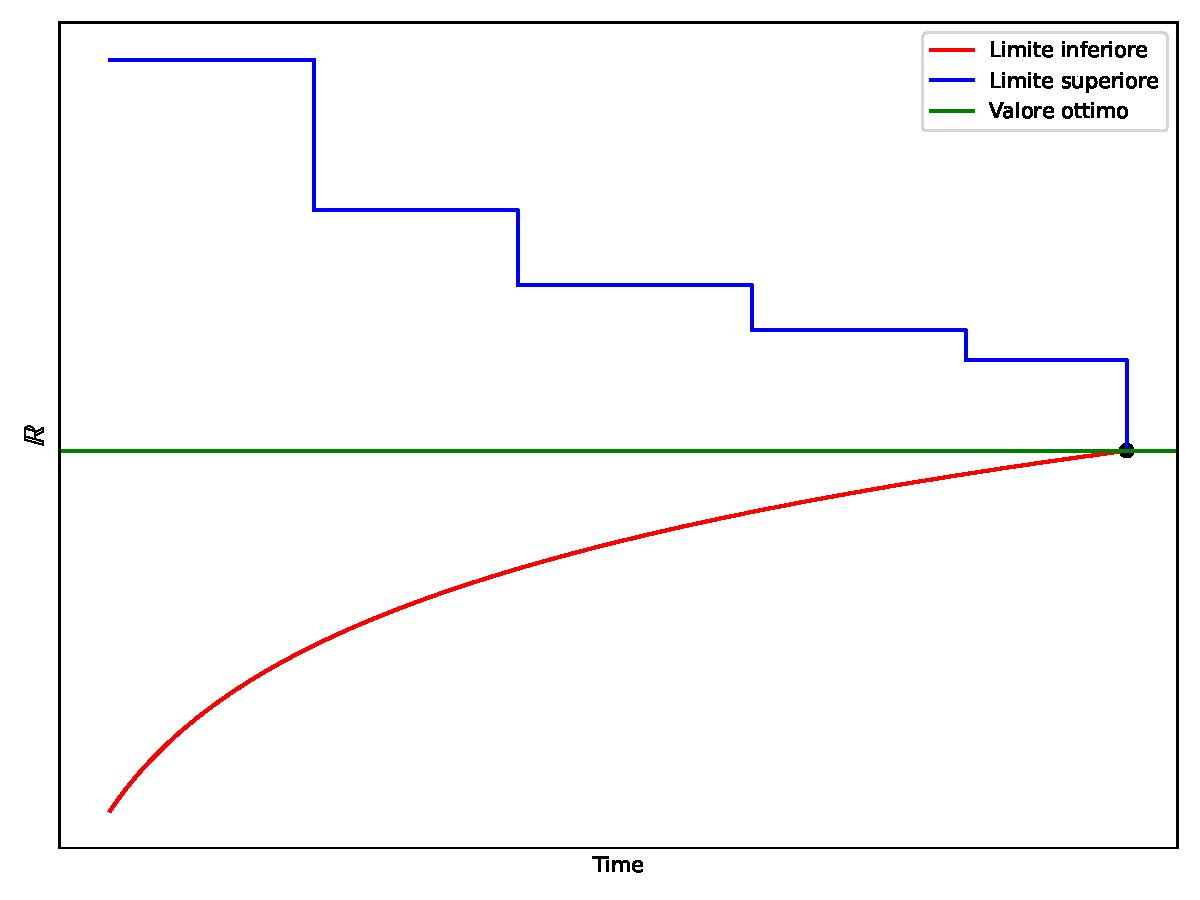
\includegraphics[scale=0.6]{img/upper_lower}
    \caption{Andamento nel tempo del limite inferiore e superiore sul 
    valore ottimo nel B$\&$B.}
\end{center}
\end{figure}

\begin{figure}[ht!]
\begin{center}
    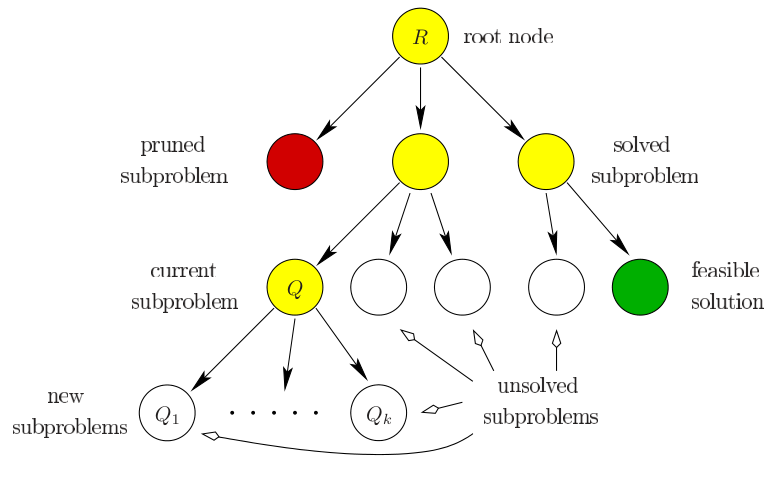
\includegraphics[scale=0.5]{./img/branchandbound.png}
\end{center}
\caption{Ricerca ad albero di un algoritmo B\&B}
\end{figure}

% TODO: Metto la parte sul B&C? Io due righe le scrivo in caso poi le tolgo.
\subsection{Algoritmo Branch and Cut}%
\label{sub:Algoritmo Branch and Cut}
L'algoritmo B\&C è stato sviluppato appositamente per risolvere i problemi di
programmazione lineare intera mista. % Cita il prof
Rispetto al B\&B, nel B\&C vengono ricavati dei piani di taglio per ogni
rilassamento lineare di ogni sottoproblema dell'albero.
Si parla di rafforzamento del rilassamento lineare associato.
L'applicazione dei questa tecnica aumenta la possibilità di ottenere una
soluzione intera dal rilassamento lineare, allo stesso tempo permette di
ottenere un migliore limite inferiore alla soluzione ottima del problema
che stiamo risolvendo.

\begin{figure}[ht!]
\begin{center}
    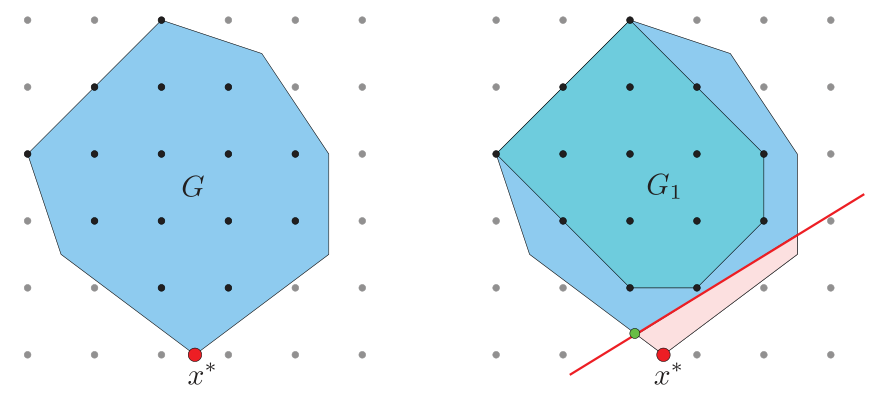
\includegraphics[scale=0.35]{img/branchandcut}
\end{center}
\caption{Applicazione di un piano di taglio dal punto di vista della regione
ammissibile}
\end{figure}

\section{Alternating Criteria Search}%
\label{sec:Alternating Criteria Search}
L'ACS è un algoritmo euristico che opera su problemi MIP.
Il suo obiettivo principale non è quello di trovare una soluzione ottima ma
di trovarne una ammissibile che abbia una buona qualità.
L'approccio utilizzato dall'ACS è quello di risolvere, in maniera iterativa,
molteplici \emph{sub-MIP} ricavati a partire dal problema principale.
I sub-MIP considerati appartengono ad una delle seguenti due tipologie:
\begin{itemize}
    \item \emph{FMIP}: questi problemi puntano a minimizzare il grado
        dell'inammissibilità della soluzione.
    \item \emph{OMIP}: questi problemi condividono la stessa funzione obiettivo
        del MIP di partenza e puntano ad ottimizzare il valore della soluzione.
\end{itemize}
Allo scopo di raggiungere questi due obiettivi, vengono risolte delle
varianti dei sub-MIP in cui un certo numero di variabili vengono fissate.
